\documentclass[fleqn]{article}
\usepackage{xcolor}
\usepackage{amsmath}
\usepackage{graphicx}
\title{Week 1 Computer Vision Notes}
\date{3-25-2020}
\author{Maxwell Li}

\begin{document}
  \color{black!20!white}
  \pagecolor{black!70!white}

  \maketitle
  \tableofcontents
  \setcounter{secnumdepth}{0}
  \newpage
  \pagenumbering{arabic}

  \section{\textbf{Section 1: Getting Started with Images}}
    \subsection{Introduction}
    Some things we will learn\\
    \quad - What is color?\\
    \quad - How does a camera see an image?\\
    \quad - How to read/write images?\\
    \quad - How to manipulate pixels?\\
    \quad - Alot more!

    \subsection{How is An Image Formed}
    Throughout history the phenomena of imaging has been explored by many ancient civilizations. The most used primitive form of a camera that has been used was the pinhole camera. The pinhole camera works by taking the light waves that bounce off of an object and projecting them through a small hole.

    \begin{figure}[h!]
      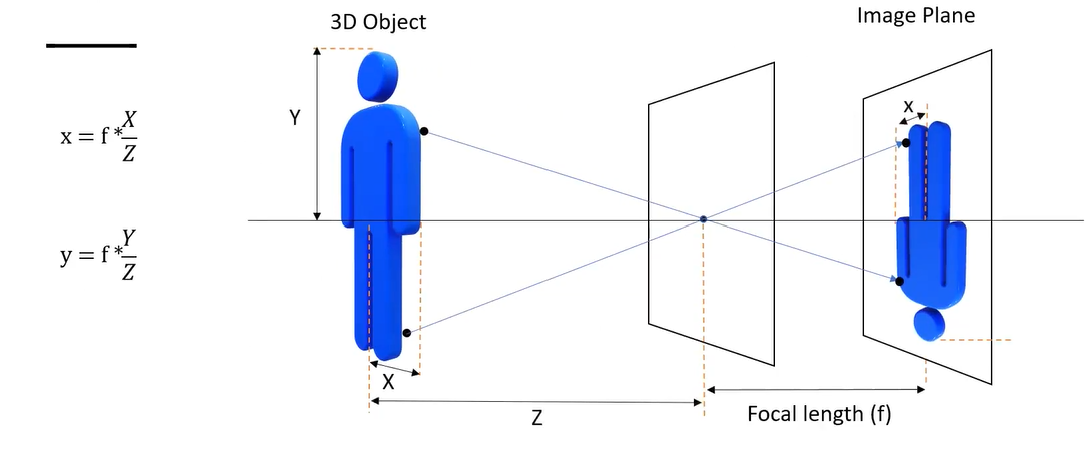
\includegraphics[width=\linewidth]{pinholecamera.png}
      \caption{PinHole Camera Example}
      \label{fig: Pinhole Camera}
    \end{figure}


\end{document}
